\chapter{A Normalized Subset of the C and C++ Languages}\label{chap:subset}

As we explored earlier in this work, two factors predominate in providing researchers and developers with a powerful and ergonomic program optimization platform.

The first, the tooling's ability to provide simple, yet powerful abstractions for querying and manipulating the programs, is arguably tackled, even if not yet completely, by the use of Clava, with its simple model and straightforward scripting in a high-level language.

However, the other predominant aspect, one that goes under-appreciated, is ensuring that the level of abstraction of the representation used is appropriate for the task at hand. This requires balancing parsimony - making sure that only the language elements that are needed to represent the domain are exposed, and no more - and expressiveness - exposing a set of language elements that is rich enough to represent the domain in a natural and concise way. The balance between the two factors naturally depends on the task. Let us consider two  examples that typify opposite ends of this balance.

\begin{itemize}
    \item A refactoring tool will find itself needing an extremely expressive intermediate representation. This stems from the overwhelming need to preserve most of the syntactic structure of the original program, compared to the relatively local kinds of changes that will be performed (such as renaming the occurrences of a variable, or extracting a method out). In extreme cases, even spacing, line breaks and indentation must be preserved, so corresponding elements must be present in the internal language.
    \item On the other hand, the middle and back-ends of a standard compilers may admit and use a much more restricted set of elements in their intermediate representation. This occurs because the target language is not meant for human consumption and is itself quite parsimonious, and because simpler languages are often easier to statically analyze, since structural pattern matching must account for a smaller set of elements and their combinations.
\end{itemize}

By analysing the use case that we tackle: supporting ergonomic, automatic yet inspectable research and implementation of program optimization, we are able to establish a set of principles to navigate this trade-off, and to present a \textit{normalized} or \textit{canonical} subset of the C and C++ languages to use as our intermediate representation.

This chapter presents these underpinning principles, and contributes a set of transformations that may be applied to reach our normalized subset.

\section{Simplified, but structured, control flow}\label{sec:subset-control-flow}

The first set of complexities that were tackled is the diverse set of control flow constructs. Control flow in C and C++ is performed by using several different statements, which can be categorized further into several categories:

\begin{enumerate}
    \item Selection statements
    \item Iteration statements
    \item Unstructured control flow statements
\end{enumerate}

For each of these categories, we considered whether the corresponding statements could be replaced with a set of patterns using fewer primitives, while rejecting the goal of replacing structured control flow statements with equivalent patterns made of unstructured control flow statements.

\subsection{Selection statements}

C and C++ use the if-statement as the main pattern for structured selection control flows. This statement takes an expression as a condition, and, depending on it evaluating to a non-zero (\textit{truthy}) or zero (\textit{falsy}) value, it will execute the statement contained in a respective statement (termed as the \textit{then} or \textit{else} branch of the statement). We consider this statement the main candidate for being the target of normalization of other selection statements.

The language allows several expressive liberties to be taken when using this statement, so Clava already performed several normalization steps for this statement. Specifically:

\begin{itemize}
    \item A branch of this statement could be a single statement, or a compound statement (a scope, denoted by the use of curly brackets around one or more inner statements). Clava automatically inserts a scope around single statements.
    \item The else branch is optional. In that case, no statement would be executed if the condition was falsy. Clava automatically inserts an empty scope for that branch.
\end{itemize}

This means that a code like:

\begin{lstlisting}[language=C]
if (condition) singleStatement();
\end{lstlisting}

Is transformed into the code:

\begin{lstlisting}[language=C]
if (condition) {
  singleStatement();
} else {}
\end{lstlisting}

Furthermore, the ternary operator can be considered a selection statement as well. As with the if-statement, this operator takes an expression as a condition, and evaluates to different expressions depending on whether the condition evaluates to a truthy or falsy value.

We aimed to rewrite this operator in terms of the if statement, and so implemented the transformation \verb|clava.code.SimplifyTernaryOp| to do so automatically. Leading the following code:

\begin{lstlisting}[language=C]
condition ? trueExpr : falseExpr;

a_type result = condition ? trueExpr : falseExpr;
\end{lstlisting}

To be transformed into:

\begin{lstlisting}[language=C]
if (condition) {
  trueExpr;
} else {
  falseExpr;
}

a_type result;
if (condition) {
  result = trueExpr;
} else {
  result = falseExpr;
}
\end{lstlisting}

This transformation furthermore requires that non-linear control flow in evaluated expressions is performed explicitly, as detailed in \ref{sec:subset-expressions}, so as to have ternary operators be placed in top-level statements or as the right hand side of a top-level assignment.

Finally, we must consider the existence of the switch (case) statement, which evaluates a condition and jumps to an execution path based not on the truth value of a condition, but by comparing it to a set of values (the cases of the statement). However, this statement, in C and C++, does not exhibit structured control flow by default, since in the absence of a break statement, the flow of execution falls through to the code path of subsequent cases in the code. It is however possible to devise a transformation that, based on analysing the existence or nonexistence of break statements and using code duplication, could guarantee structured control flow in these cases, transforming code such as:

\begin{lstlisting}
switch (cond) {
  case 1:
    stmt1_1;
    stmt1_2;
  case 2:
    stmt2;
    break;
  case 3:
    stmt3;
}
\end{lstlisting}

Into code like:

\begin{lstlisting}
switch (cond) {
  case 1: {
    stmt1_1;
    stmt1_2;
    stmt2;
    break;
  }
  case 2: {
    stmt2;
    break;
  }
  case 3: {
    stmt3;
    break;
  }
}
\end{lstlisting}

allowing the switch statement to be subsequently transformed into a chain of if statements:

\begin{lstlisting}
if (cond == 1) {
  stmt1_1;
  stmt1_2;
  stmt2;
} else if (cond == 2) {
  stmt2;
} else if (cond == 3) {
  stmt3;
}
\end{lstlisting}

The main factor that complicates this transformation is that there is no guarantee that the control flow in a switch statement is structured. For example, one could have case labels in between components of an if statement, or a Duff's device \cite{Duff1988}, or declarations that are unreachable for a label but reachable code that nevertheless uses said declarations. Therefore, it was infeasible, at least for the scope of this work, to devise a general transformation for this case. We also decided to de-prioritize work on a restricted version of it, so no attempt was made at such implementation.

\subsection{Iteration statements}\label{sec:subset-iteration}

Iteration statements are statements where a condition is repeatedly evaluated, and a set of statements are executed as long as the condition holds. The C and C++ languages define four types of statement to perform this control flow: the while statement, the do-while statement, the traditional (three statement) for statement, and the range or iterator-based for statement (for-each statement, in our parlance).

While these statements could be rewritten in terms of selection statements and unconditional jumps, the pattern of iteration is important enough to warrant explicit expression, and at least one of the iteration statements should be kept. Thus we chose to keep as a primitive the while statement, which is the conceptually simpler of the four. The while statement evaluates the condition at the \textbf{beginning} of each iteration and executes the body if the condition holds true.

The other conceptually simple statement is the do-while statement. The do-while statement evaluates the condition at the \textbf{end} of each iteration, and so is guaranteed to execute \textit{at least one} iteration.

The processes for transforming a while statement into a do-while statement and vice-versa are well known. To transform a while statement into a do-while statement we would perform a \textit{loop inversion}: replace the while statement with a do-while statement, and wrap it in an if statement, duplicating the condition. This inversion often proves to be worthwhile in terms of performance, since it reduces the number of branches, which predominates over the duplicated code to calculate the condition.

However, we find that while statements are generally more used and better understood, so we implemented instead the transformation \verb|DoToWhileStmt|, which transforms a do-while statement to a while statement by peeling the first iteration in a separate scope before the transformed loop, transforming code such as:

\begin{lstlisting}
stmt0;
do {
  stmt1;
  stmt2;
} while(cond);
\end{lstlisting}

Into code like:

\begin{lstlisting}
stmt0;
{
  stmt1;
  stmt2;
}
while(cond) {
  stmt1;
  stmt2;
}
\end{lstlisting}

While this transformation results in more duplicated code, we believe that its expected infrequency compared to the reverse transformation makes it more desirable.

The next element to consider is the for statement. This statement allows the user to concisely define a canonical loop by having the usual steps of it (declaring the inductive variable, expressing the loop condition, and stepping the inductive variable) all present in the loop header. However, to maintain our desirable degree of parsimony, we implemented the \verb|ForToWhileStmt| transformation, which extracts out the initialization and step sub-statements and transforms the for statement into a while statement, turning code like:

\begin{lstlisting}
for (init; cond; step) {
  stmt1;
  stmt2;
}
\end{lstlisting}

Into:

\begin{lstlisting}
{
  init;
  while (cond) {
    stmt1;
    stmt2;
    
    step;
  }
}
\end{lstlisting}

Finally, we considered the C++-only 'range-based for statement', or for-each statement for short. This statement can be converted in a straight-forward manner to a for statement, according to the C++ standard:

\begin{quote}
The range-based for statement

\verb|for (init-statement for-range-declaration : for-range-initializer)|
\verb|  statement|

is equivalent to
\begin{verbatim}
{
  init-statement
  auto &&range = for-range-initializer ;
  auto begin = begin-expr ;
  auto end = end-expr ;
  for ( ; begin != end ; ++begin ) {
    for-range-declaration = * begin ;
    statement
  }
}
\end{verbatim}
\end{quote}

Following that, it could be further rewritten in terms of a while statement. We did not implement this transformation, since we considered it to be of low priority in a prototypical implementation.

\subsection{Unstructured control flow}

The last category of statements that we considered were unstructured control flow statements:

\begin{itemize}
    \item Break statements
    \item Continue statements
    \item Early return statements
    \item Exception throwing and catching
    \item Long jumps
    \item Go-to statements
\end{itemize}

These statements, in the general case, cannot be converted to equivalent structured statements without introducing meaningfully complex code changes and/or auxiliary variables, so we decided against implementing transformations to remove them. Two exceptions were made against this decision.

Firstly, in the case where for statements were converted to while statements, it was necessary to transform continue statements into equivalent go-to statements to a label before the step expression at the end of the loop.

Secondly, a transformation to remove early returns from a function, by introducing unconditional jumps to the end of a function and the use of an auxiliary variable, was developed, for use in specific applications (such as function inlining).

\section{Explicit side-effects and transfers of control flow in expression evaluation}\label{sec:subset-expressions}

C and C++ allow the building of arbitrarily complex expressions to be evaluated during execution, expressions which may contain elements in their construction that perform side-effects or transfer control flow in some way.

Some examples of this complexity may include divergent control flow in evaluation, such as when using ternary operators, side-effects during expression evaluation, such as when evaluating assignments and unary increment and decrement operators, and potentially interprocedural jumps, such as when evaluating a call or a throw.

In many situations, when performing analyses, it is useful to separate these complexities from the comparatively mundane calculations that may be performed around them.

Furthermore, we found that, when performing some transformations, such as function call inlining, there were cases where we would need to place several statements in a place that only accepted a single expression, and so it would be useful to separate the complex steps of a certain expression's evaluation from its use, in order to simplify implementation.

Therefore, we aimed to restrict the expression syntax to a more manageable set of elements. Specifically, we decided that any use of an expression (such as in a call parameter or in a header of a selection or iteration statement) could only be made with an immediate or an existing variable, and that the evaluation of any complex expression ought to be simplified by using one or more temporary variables, according to the following rules - the rvalue of a variable assignment can be:

\begin{itemize}
    \item An immediate or an existing variable.
    \item One or more unary operators applied in succession to an immediate or an existing variable. Unary decrement and increment operators are not allowed.
    \item A binary operator, whose arguments are an immediate, an existing variable, or another binary operator, to which this restriction on allowed arguments applies recursively. Assignment operators are not allowed.
    \item An interprocedural call, whose arguments can only be an immediate or an existing variable.
\end{itemize}

In general, these restrictions should be understood to adhere to the principle that \textit{expressions should pertain only to combinations of pre-existing and primitive values}. Other concerns should be dealt with externally to expression evaluation.

Of course, these restrictions imply that a range of valid expressions must be rewritten using our restricted set of constructs. The following subsections detail such cases, and how they were rewritten.

Other expressions need only to be decomposed. In those cases, we insert temporary variables to contain the intermediate results of those expressions' evaluation.

After this process of transformation and decomposition, we are left with a sequence of statements to be placed preceding to any place the expression is evaluated in, a new value for the expression, and a sequence of statements to be placed after the evaluation\footnotemark. These statements might be repeatedly inserted, depending on the control flow of the program (for example, in a while statement, the preceding statements will be inserted before the loop and at the end of each iteration, and the succeeding statements will be placed at the beginning of each iteration and after the loop, coinciding with the occasions where the loop condition is evaluated). \footnotetext{Strictly speaking, there is not a specific total order of evaluation, as the standards do not mandate a general order of evaluation, unless an operator with more specific semantics introduces such an order. These operators are known to introduce \textit{sequence points} into the program evaluation. Examples of such operators are: the comma operator, short-circuiting union and intersection operators, ternary operators, function calls, among others. In practice, we must serialize the order of evaluation anyway, since the program source is sequential by nature, so we serialize the expression tree left-to-right, post-order.}

\subsection{Explicit side-effect evaluation}

There are several expressions in C and C++ that can also effect changes on the global state. These expressions, while useful when writing expressive, high-level code, can complicate reasoning about the program automatically, since, for a single expression, both value production and side-effects must be tracked. Therefore we aim to rewrite these expressions to separate value computation and side-effect application.

The first kind of expressions that needed to be rewritten were the ones that performed side-effects on the variables they were operating on. These were assignment operators and unary increment and decrement operators. These operators, while returning a value, simultaneously mutate a variable. Separating this mutation is useful to allow analyses to reason about the mutation separately, and to be able to assume that expression evaluation is a pure computation.

Therefore, we devised transformations to insert a separate statement performing the mutation, and to reference the results of the mutation explicitly, according to the semantics of each operator:

\begin{itemize}
    \item When evaluating an assignment operation, the assignment will be performed in a previous statement, and the lvalue of the assignment will be subsequently used in the computed expression.
    \item When evaluating a pre-increment or pre-decrement unary operator, the increment or decrement will be inserted before the expression evaluation, and the target will be used in the computed expression.
    \item When evaluating a post-increment or post-decrement unary operator, the target will be used in the computed expression, and the operation will be inserted as a subsequent statement.
\end{itemize}

This means that code like:

\begin{lstlisting}
int a = 1;
int i = 2;
int j = 3;

int b = (a += i++ + ++j);
\end{lstlisting}

Will be rewritten to:

\begin{lstlisting}
int a = 1;
int i = 2;
int j = 3;

++j;
a += i + j;
int b = a;
i++;
\end{lstlisting}

Afterwards, the isolated unary increment and decrement operators can safely be rewritten to a simple assignment with a sum.

\subsection{Explicit transfers and divergences in control flow}

We also strive to make complex control flow more explicit. 

Firstly, calls are isolated from other elements of the expression:

\begin{lstlisting}
int a = f(b, g(c, d);

// becomes

int temp0 = g(c, d);
int a = f(b, temp0);
\end{lstlisting}

Secondly, ternary operators are completely removed and rewritten in terms of an if-statement, after they are separated from the rest of the expression evaluation:

\begin{lstlisting}
int a = conditionA ? (conditionB ? expr1 : expr2) : expr3;

// becomes

int a;
if (conditionA) {
  if (conditionB) {
    a = expr1;
  } else {
    a = expr2;
  }
} else {
  a = expr3;
}
\end{lstlisting}

Another relevant transformation, that was not implemented and is left as future work, is rewriting short-circuiting boolean operators with if statements, so as to preserve the sequencing and conditional execution properties of the operator when the operators are decomposed. This would mean that a statement such as:

\begin{lstlisting}
bool condition;
condition = (expr1 && expr2) || (expr3 && expr4);
\end{lstlisting}

Would be rewritten not as:

\begin{lstlisting}
bool condition;

bool temp1;
temp1 = expr1;
// semantic error: executes side-effects of `expr2` when `expr1` evaluates to false
bool temp2;
temp2 = expr2;
bool temp1and2;
temp1and2 = temp1 && temp2;

// semantic error: executes side-effects of `expr3 && expr4` when `expr1 && expr2` evaluates to true
bool temp3;
temp3 = expr3;
// semantic error: executes side-effects of `expr4` when `expr3` evaluates to false
bool temp4;
temp4 = expr4;
temp3and4 = temp3 && temp4;

condition = temp1and2 || temp3and4;
\end{lstlisting}

But as:

\begin{lstlisting}
bool condition;
{
  bool tempUnion;
  {
    bool temp1and2;
    {
      temp1and2 = expr1;
    }
    if (temp1and2) {
      // correct: only executes side-effects of `expr2` when `expr1` evaluates to true
      temp1and2 = expr2;
    }
    tempUnion = temp1and2;
  }
  if (!tempUnion) {
    // correct: only executes side-effects of `expr3 && expr4` when `expr1 && expr2` evaluates to false
    bool temp3and4;
    {
      temp3and4 = expr3;
    }
    if (temp3and4) {
      // correct: only executes side-effects of `expr4` when `expr3` evaluates to true
      temp3and4 = expr4;
    }
    tempUnion = temp3and4;
  }
  condition = tempUnion;
}
\end{lstlisting}

A final transformation that was left unimplemented was removing the comma operator, which would transform code like:

\begin{lstlisting}
// void side_effect(int *n);
// int arg;
int n;
n = side_effect(&arg), arg;
\end{lstlisting}

Into:

\begin{lstlisting}
// void side_effect(int *n);
// int arg;
int n;
side_effect(&arg);
n = arg;
\end{lstlisting}

\section{Overall simplification of the language and removal of superfluous elements}

Besides the two kinds of simplification detailed in the two previous sections, we defined a further set of simplifications to be made to the language. They consist of rote substitutions of convenience operators for their more verbose primitive versions, and other simple transformations. These include:

\begin{itemize}
    \item Breaking up variable declaration statements into several statements, to ensure that only one variable is declared in each statement.
    \item Separating variable initialization from variable declaration, by placing the initial value in a separate assignment statement.
    \item Removing complex assignment operators, by replacing with assignments whose rvalue is the primitive operator corresponding to the complex assignment. E.g, \verb|a += 1| becomes \verb|a = a + 1|. Exceptions regarding side-effecting lvalue calculations and atomic lvalues are not implemented, and left as future work.
    \item Removing variable declarations the condition statements in the headers of selection and iteration statements. Not implemented.
    \item Removing variable shadowing. When variables are declared in inner scopes with the name of an existing variable in an outer scope, they are renamed to avoid shadowing it.
\end{itemize}

\section{Schedule of transformations}

After considering the goals for our intermediate language, defined as a subtractive subset of the existing C and C++ languages, we now can define a schedule of transformation passes, to be applied to a program written in these languages, that normalizes it to an equivalent program in our language subset:

\begin{enumerate}
    \item Break up variable declarations, separate variable declarations from their initialization
    \item Rewrite all loops in terms of while statements.
    \item Separate variable declarations from condition statements in the headers of selection and iteration statements.
    \item Decompose and simplify all complex expressions.
    \item Rewrite any remaining ternary operators in terms of if statements.
    \item Smaller simplifications, e.g. remove complex assignment operators, remove variable shadowing.
\end{enumerate}

\begin{figure}
    \centering
    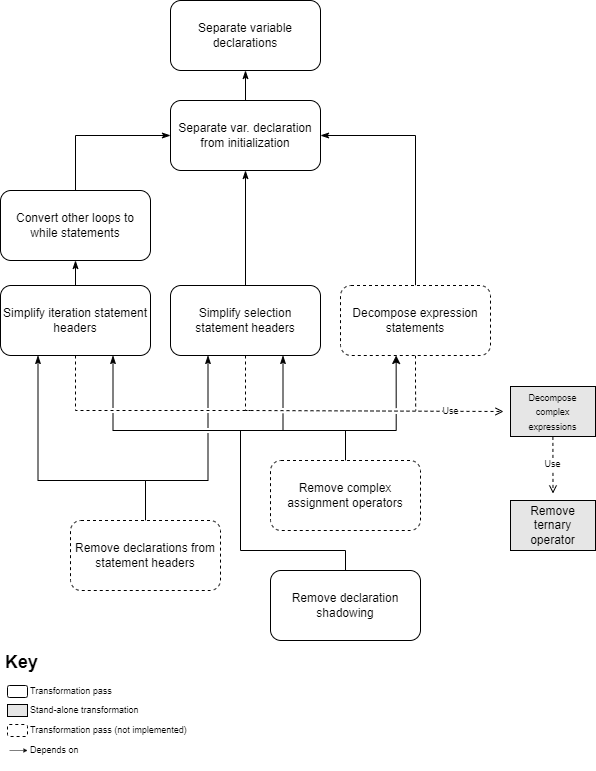
\includegraphics[width=\textwidth]{transformations.png}
    \caption{Dependency diagram of the envisioned transformations, their implementation status, and auxiliary transformations.}
    \label{fig:transform-diagram}
\end{figure}

Figure \ref{fig:transform-diagram} illustrates the dependencies between each transformation. Furthermore, because not all transformations were implemented, their implementation status is made explicit. Finally, we show where some auxiliary transformations are used.

After these transformations, we come to have a normalized program that is ready for further analyses and optimizations to be applied.

\section{Conclusion}

In this chapter we have discussed the factors that lead compiler developers to opt for more or less complex intermediate languages, outline the two main goals for our intermediate language - simplified but structured control flow, and explicit separation of expression value, control flow and side-effect evaluation - and their implications, and contribute a schedule of transformations that, when applied to a program, yield an equivalent program in a normalized subset of the source language.
